\chapter{Weitere Aspekte}
\label{ch:additional_aspects}

\section{Plattform absichern}
\label{sec:secure_platform}
\subsection{Allgemeines}
Die forensische Analyseplattform muss besonders gegen unbefugten Zugriff gesichert werden, da bei forensischen Analysen unter anderem personenbezogene Daten, aber auch Geschäftsgeheimnisse aus dem kommerziellen Umfeld, verarbeitet werden. Hierbei wäre es absolut untragbar, wenn Unbefugte die Daten lesen oder sogar modifizieren könnten.\\

\noindent
Im Hadoop-Umfeld existieren hierzu bereits Lösungen, wie Daten vor unbefugtem Zugriff geschützt werden können. Das Absichern des Clusters bezieht sich primär auf die Nutzung von Kerberos zur Authentifizierung. Es gibt einige weitere Projekte, wie beispielsweise Apache Ranger, Apache Atlas und Apache Knox, die zum Absichern des Clusters integriert werden können. Sie alle adressieren einen bestimmten Aspekt zur Verbesserung der Systemsicherheit. Nachfolgend soll die Authentifizierung mit Kerberos erklärt werden und Möglichkeiten zur Datenverschlüsselung aufgezeigt werden. Die hier entwickelte forensische Analyseplattform nutzt derzeit weder eine Authentifizierung noch ist eine Datenverschlüsselung vorhanden. Allerdings können diese Aspekte in einer zukünftigen Weiterentwicklung implementiert werden.

\subsection{Authentifizierung}

Im Produktivbetrieb wird ein Hadoop-Cluster normalerweise in Kombination mit Kerberos verwendet, um einen allgemeinen Zugriffsschutz zu ermöglichen.\cite{hadoop_security} Nicht nur Apache Hadoop selbst, sondern auch alle verwendeten Projekte aus dem Hadoop-Ökosystem müssen die Nutzung mit Kerberos unterstützen. Ein Großteil dieser Projekte unterstützt dies auch. Gerade bei den hier genutzten Projekten, wie Apache Spark, Apache HBase und Apache Solr wurde daher darauf geachtet, dass diese mit Kerberos genutzt werden können.\\

\noindent
Kerberos ist ein kryptografisches Netzwerkprotokoll, welches basierend auf Tickets den Authentifizierungsprozess gegenüber mehreren Servern vereinfachen soll (\textit{Ticket Single Sign-On}).\cite[S. 425-429]{crypto}\\
Das grundlegende Problem, welches dieses Protokoll löst, ist der erhöhte Verwaltungsaufwand bei der Authentifizierung gegenüber einer Systemlandschaft aus mehreren Servern. Prinzipiell besteht das Hadoop-Cluster aus mehreren Knoten, auf welchen unterschiedliche Services angeboten werden. Bei der forensischen Analyseplattform könnte der Nutzer Daten aus dem HDFS, HBase oder Solr auslesen, eine Datenverarbeitung mit Apache Spark ausführen oder die allgemeine Ressourcenauslastung des Systems anzeigen. Für all diese Aktionen sind unterschiedliche Services und Komponenten verantwortlich. Ist das System vollständig abgesichert, müsste sich der Nutzer vor jeder Nutzung bei jedem Service getrennt authentifizieren (beispielsweise mittels Nutzername und Passwort). Darüber hinaus müssten sich auch die Komponenten untereinander authentifizieren, denn Apache Spark greift bei der Datenverarbeitung auf die Daten im HDFS zu und schreibt wiederum Daten in HBase. Um diesen Authentifizierungsaufwand zu verringern, wurde Kerberos entwickelt. 
Bei Kerberos existiert ein zentraler Authentifizierungsserver, gegenüber dem sich ein Nutzer authentifizieren muss. Dieser Server ermöglicht mithilfe sogenannter Tickets die temporäre Authentifizierung gegenüber aller anderen Server, auf welche der Nutzer zugreifen darf.\cite[S. 425-429]{crypto} Abbildung \ref{fig:kerberos} skizziert dieses Verfahren. 
\begin{figure}[ht]
  \centering
  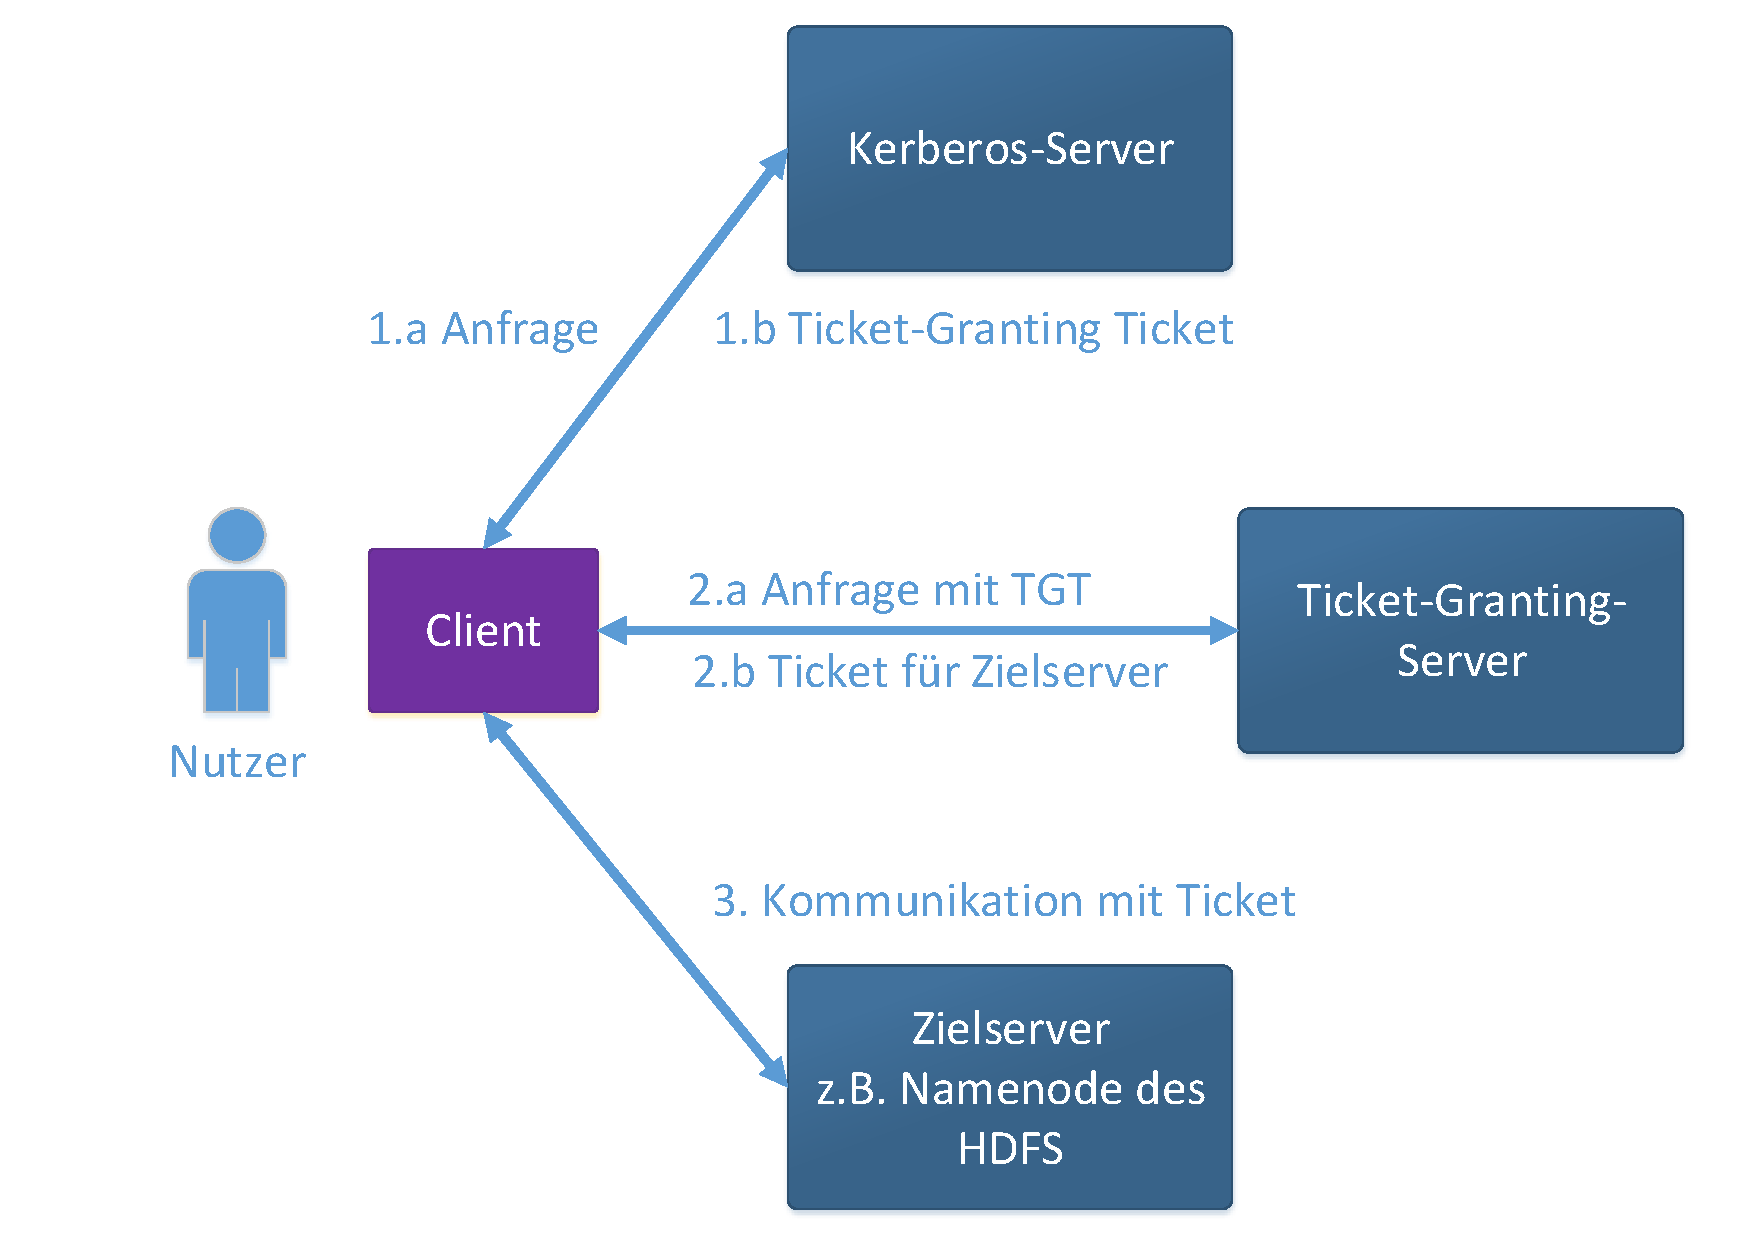
\includegraphics[width=0.9\textwidth]{./resource/kerberos_authentification.pdf}
  \caption{Authentifizierung mit Kerberos (Vgl. \cite[S.426]{crypto})}
  \label{fig:kerberos}
\end{figure}

\noindent
Zu Beginn sendet der Nutzer eine Anfrage an den Kerberos-Server zur Authentifizierung (zum Beispiel mit Nutzername und Passwort). Danach erhält dieser vom Server ein sogenanntes \textit{\gls{tgt}}. Mithilfe des TGT kann er nun beim \gls{tgs} Tickets für spezifische Zielserver und Services anfordern. Mit einem Ticket für einen konkreten Server oder Service kann der Client nun eine verschlüsselte Verbindung mit dem Zielserver öffnen.\\
Ein Ticket ist letztlich ein verschlüsselter Datensatz mit Nutzername und Zugangsberechtigungen für einen spezifischen Server. Der Zielserver kann die für den Server erstellten Tickets vom Ticket-Granting-Server entschlüsseln und so sicherstellen, dass sich der Nutzer authentifiziert hat. Der Ticket-Granting-Server wird bei Kerberos genutzt, um das Schlüsselmanagement sicherer zu machen. Denn dieses Ticket-Granting Ticket ist nur für eine begrenzte Zeit gültig und muss dann wieder neu angefordert werden. Hierdurch ist es für einen Angreifer schwerer, dauerhaften Zugriff auf die Services zu erhalten, falls dieser den Sitzungsschlüssel des Ticket-Granting Tickets ermitteln kann.\cite[S. 425-429]{crypto}\\

%Eine Alternative könnte hier auch Cloudera Sentry, Apache Ranger, Apache Atlas oder Apache Knox\footnote{https://knox.apache.org/} sein.

\subsection{Datenverschlüsselung}
Zum Schutz der Daten im Hadoop-Cluster können diese verschlüsselt werden. Hierbei kann zwischen der \textit{Persistenzverschlüsselung} und \textit{Transportverschlüsselung} unterschieden werden. Die Persistenzverschlüsselung kann auf unterschiedlicher Ebene durchgeführt werden. Es ist möglich die Festplatten aller Knoten im Hadoop-Cluster auf Betriebssystemebene zu verschlüsseln. Hier könnte das sogenannte \textit{\gls{luks}} auf Linux-basierten Betriebssystemen genutzt werden, um die Festplatten und alle darauf gespeicherten Daten zu verschlüsseln. Diese Art der Verschlüsselung ist unabhängig vom Hadoop-Ökosystem und sichert daher alle Daten auf den Knoten. Allerdings ist die Verwaltung aufwendig, da beim Ersetzen von Festplatten oder dem Hinzufügen neuer Knoten die Verschlüsselung nochmals durchgeführt werden muss. Darüber hinaus müssen bei einem Neustart der Knoten auch die Passwörter zur Entschlüsselung angegeben werden. Hierzu gibt es aber auch spezifische Komponenten, die die Verwaltung der Schlüssel übernehmen. \cite[S. 202-204]{hadoop_security}\\

\noindent
Ein anderer Ansatz ist die Verschlüsselung der Daten auf Applikationsebene. Beim HDFS besteht die Möglichkeit sogenannte \textit{Verschlüsselungszonen (Encryption Zones)} zu nutzen. Dabei werden schon auf Anwendungsebene die Daten verschlüsselt im HDFS abgelegt. Darüber hinaus besteht durch die Nutzung mehrerer Verschlüsselungszonen auch die Möglichkeit, die Daten innerhalb des HDFS nochmals gegen ungewollte Nutzerzugriffe zu sichern. Dies kann beispielsweise die Sicherheit bei der Speicherung von Daten unterschiedlicher Firmen im gleichen HDFS erhöhen. Um die Daten zu entschlüsseln, wird bei dieser Variante ein unabhängiger Schlüsselserver benötigt, der einem Nutzer die entsprechenden Schlüssel abhängig von seinen Zugangsberechtigungen bereitstellt. Zusätzlich existiert ein sogenannter \textit{Hadoop Key Management Server}, welcher die Kommunikation zwischen Client, HDFS und Schlüsselserver steuert.\cite[S. 192-200]{hadoop_security}
Diese Variante zur Datenverschlüsselung bezieht sich allerdings nur auf das HDFS. Bei der Datenverarbeitung im Hadoop-Umfeld können aber auch Daten temporär zwischengespeichert werden. Diese wiederum werden nicht von der Datenverschlüsselung im HFDS abgedeckt und könnten somit ungeschützt auf den einzelnen Knoten im Cluster gespeichert sein. Hier zeigt sich, dass die Absicherung im Hadoop-Cluster immer auch spezifisch für die genutzten Komponenten geprüft werden. \\

\noindent
Auch die Transportverschlüsselung im Hadoop-Cluster sollte betrachtet werden, da hier einerseits sensible Daten zwischen den Knoten aber auch von einzelnen Knoten zu den Rechnern der Nutzer transportiert werden müssen. Bei Webservices über HTTP sollte daher die Verschlüsselung mittels \textit{\gls{tls}} durchgeführt werden. Darüber hinaus bietet Apache Hadoop weitere Möglichkeiten, um auch die Kommunikation zwischen den Knoten entsprechend zu verschlüsseln. Auch hier reicht es nicht aus, nur Apache Hadoop zu betrachten, sondern auch alle anderen Komponenten, die im Hadoop-Cluster arbeiten. \cite[S. 207-216]{hadoop_security}\\

\noindent
In der aktuellen Analyseplattform wird derzeit keine Datenverschlüsselung oder Transportverschlüsselung eingesetzt. Zumindest die Transportverschlüsselung sollte in einer zukünftigen Weiterentwicklung implementiert werden, um die Datensicherheit über das Netzwerk zu erhöhen.

\section{Datenlöschung}
Auch das forensisch korrekte Löschen der Daten, nach der Fallanalyse muss betrachtet werden. Bei einer forensischen Analyse werden die Asservate sichergestellt und für einige Zeit verwahrt. Die Computersysteme, mit welchen die Daten analysiert und verarbeitet werden, müssen bereinigt werden. Diese Bereinigung wird meistens durch das mehrmalige Überschreiben der persistenten Datenträger gewährleistet.\\
 Im Hadoop-Umfeld ist dieses Vorgehen aufwendiger. Es ist zwar möglich mit der hier entwickelten Datenimport-Anwendung aus Kapitel \ref{subsec:data_import_implementation} die Daten aus dem HDFS und HBase zu löschen. Allerdings bedeutet dies noch lange nicht, dass sich keine Datenrückstände auf den Festplatten der einzelnen Knoten befinden.
Für gewöhnlich werden die Daten im HDFS über einen längeren Zeitraum gespeichert und müssen nicht forensisch korrekt gelöscht werden. Daher ist es nachvollziehbar, dass im Hadoop-Ökosystem dieser Aspekt bisher nicht ernsthaft betrachtet wurde.\\

\noindent
Das Projekt \textit{\gls{sdhdfs}} versucht diesen Aspekt zu berücksichtigen und implementiert einen eigenen Mechanismus zum Löschen von Daten im HDFS.\cite{sd_hdfs} Hierbei werden die allokierten Datenblöcke im HDFS auf den einzelnen Knoten überwacht. Die Datenblöcke, welche aus dem HDFS gelöscht wurden, werden mehrmals mit zufällig generierten Daten überschrieben. 
Allerdings ist es fraglich, ob dieser Ansatz wirklich funktioniert. Denn je nach konkretem Speichertyp, ist durch das bloße Überschreiben auf Betriebssystemebene nicht gewährleistet, dass die Daten auch wirklich auf der Festplatte überschrieben werden. 
Dies wäre zum Beispiel der Fall bei SSDs. Ein weiterer Punkt ist auch, dass im Hadoop-Umfeld die Daten nicht ausschließlich im HDFS abgespeichert werden. Beispielsweise könnten Teile der Metadaten in Log-Dateien enthalten sein oder in temporären Dateien zwischengespeichert werden. So können bei Apache Spark nach Bedarf auch Zwischenergebnisse persistent auf die Festplatte ausgelagert werden.\cite{spark_rdd} Diese Daten werden bei dem Ansatz von SD-HDFS nicht berücksichtigt. Darüber hinaus scheint dieses Projekt nicht mehr weiter verfolgt zu werden, da kaum Informationen zu dessen Einsatz bekannt sind.\\

\noindent
Die  derzeit einzige forensisch korrekte Lösung ist die Datenlöschung aller Datenträger. Dies bedeutet jedoch auch die Neuinstallation des Analysesystems auf allen Knoten. Aber nur dadurch könnte sichergestellt werden, dass temporäre Datenfragmente garantiert gelöscht sind.  